
\documentclass[11pt,a4paper]{report}

\usepackage[portuges]{babel}
\usepackage[utf8]{inputenc} % define o encoding usado texto fonte (input)--usual "utf8" ou "latin1
\usepackage{graphicx} %permite incluir graficos, tabelas, figuras
\usepackage{subcaption}
\usepackage{listings}
\usepackage{color}
\usepackage{multicol}
\usepackage{indentfirst}
\usepackage{hyperref}
\usepackage{amsmath}
\usepackage{amssymb}
\usepackage{float} 

\definecolor{myblue}{rgb}{0.2,0.2,0.8}
\definecolor{mygray}{rgb}{0.5,0.5,0.5}
\definecolor{mymauve}{rgb}{0.58,0,0.82}

\lstdefinestyle{code}{ 
  backgroundcolor=\color{white},   % choose the background color; you must add \usepackage{color} or \usepackage{xcolor}; should come as last argument
  basicstyle=\footnotesize,        % the size of the fonts that are used for the code
  breakatwhitespace=false,         % sets if automatic breaks should only happen at whitespace
  breaklines=true,                 % sets automatic line breaking
  captionpos=b,                    % sets the caption-position to bottom
  commentstyle=\color{white},    % comment style
  deletekeywords={...},            % if you want to delete keywords from the given language
  escapeinside={\%*}{*)},          % if you want to add LaTeX within your code
  extendedchars=true,              % lets you use non-ASCII characters; for 8-bits encodings only, does not work with UTF-8
  firstnumber=1000,                % start line enumeration with line 1
  keepspaces=true,                 % keeps spaces in text, useful for keeping indentation of code (possibly needs columns=flexible)
  keywordstyle=\color{blue},       % keyword style
  language=C++,                 % the language of the code
  morekeywords={*,...},            % if you want to add more keywords to the set
  numberstyle=\tiny\color{mygray}, % the style that is used for the line-numbers
  rulecolor=\color{black},         % if not set, the frame-color may be changed on line-breaks within not-black text (e.g. comments (green here))
  showspaces=false,                % show spaces everywhere adding particular underscores; it overrides 'showstringspaces'
  showstringspaces=false,          % underline spaces within strings only
  showtabs=false,                  % show tabs within strings adding particular underscores
  stepnumber=2,                    % the step between two line-numbers. If it's 1, each line will be numbered
  stringstyle=\color{mymauve},     % string literal style
  tabsize=2,	                   % sets default tabsize to 2 spaces
  title=\lstname                   % show the filename of files included with \lstinputlisting; also try caption instead of title
}

\title{Sistemas Operativos - Trabalho Prático\\
       \textbf{Grupo 17}\\ Resolução
       } %Titulo do documento
%\title{Um Exemplo de Artigo em \LaTeX}
\author{Inês Pires Presa\\ (A90355)\and Ivo Miguel Gomes Lima\\ (A90214)\and Tiago dos Santos Silva Peixoto Carriço \\ (A91695)
       } %autores do documento
\date{\today} %data

\begin{document}
	\begin{minipage}{0.9\linewidth}
        \centering
		
\includegraphics[width=0.4\textwidth]{um.jpeg}\par\vspace{1cm}
                \href{https://www.uminho.pt/PT}
		{\scshape\LARGE Universidade do Minho} \par
		\vspace{0.6cm}
                \href{https://lcc.di.uminho.pt}
		{\scshape\Large Licenciatura em Ciências da Computação} \par
		\maketitle
		\begin{figure}[H]
			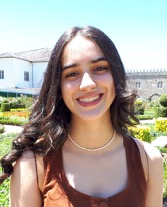
\includegraphics[width=0.32\linewidth]{ines.jpg}
			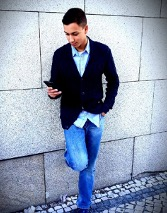
\includegraphics[width=0.32\linewidth]{ivo.jpg}
			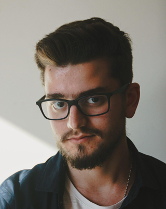
\includegraphics[width=0.32\linewidth]{tiago.jpg}
		\end{figure}
	\end{minipage}

\tableofcontents % insere Indice

\chapter{Introdução}

Foi-nos proposto, no âmbito da unidade curricular de Sistemas Operativos, o desenvolvimento de um sistema capaz de transformar vários ficheiros de áudio concurrentemente, consultar as tarefas em execução, mostrando ainda o número de filtros disponiveis e em uso nessas transformações. Este tipo de
sistema utiliza um conjunto de executáveis utilizados para filtrar e modificar um fluxo de áudios, permitindo tratar grandes quantidades de dados explorando a
concorrência entre os diferentes processos.

Neste relatório,vamos explicitar a nossa abordagem ao problema, justificando a estrutura do nosso sistema, demonstrando os
conhecimentos adquiridos durante as aulas, tais como a utilização/criação de processos, duplicação de descritores, criação de \emph{pipes} sem nome, execução de processos, aplicação de sinais e  \emph{system calls}.

\chapter{Estrutura de implementação}

\section{Cliente (\emph{aurras.c})}

\section{Servidor (\emph{aurrasd.c})}

\chapter{Funcionalidades}



\section{Filtros}

No nosso projeto quando é feita a submissão de um pedido do tipo \emph{\$ ./aurras transform samples/sample-1.m4a output.m4a ...} foi nos apresentados cinco filtros básicos que recebem o \emph{input} pelo \emph{standard input} e produzem \emph{output} para o \emph{standard output}.

\begin{itemize}
\item \emph{\textbf{aurrasd-echo}} (eco) - Este filtro
\item \emph{\textbf{aurrasd-gain-double}} (alto) - Este filtro
\item \emph{\textbf{aurrasd-gain-half}} (baixo) - Este filtro
\item \emph{\textbf{aurrasd-tempo-double}} (rapido) - Este filtro
\item \emph{\textbf{aurrasd-tempo-half}} (lento) - Este filtro
\end{itemize}

Todos estes filtros podem mudar a sua constituição (efeito e máximo de aplicações) conforme são mudados/acrescentados ficheiros presente nas pastas \emph{/bin/aurrasd-filters/} e \emph{/etc/aurrasd.conf}.

\chapter{Conclusão}

Durante a realização deste trabalho prático embora o mesmo tenha sido apelidado de simples e até mesmo básico por parte da equipa docente, sentimos que exigiu uma grande organização da nossa parte para que não fosse perdido o foco do problema que estavamos a enfrentar. Tendo a aplicação dos conceitos teóricos revelado-se, de uma maneira geral, bastante interessante e desafiante pois tal como \emph{\textbf{Ward Cunningham}} disse \emph{\textbf{It's all talk until the code runs}}. 

Uma das peças fundamentais para a concretização do projeto foram as resoluções dos guiões práticos apresentadas pela equipa de docentes e até mesmo as nossas, pois serviram de apoio para o esclarecimento de dúvidas que surgiram, o que nos permitiu finalizar o mesmo com todas as funcionalidades solicitadas. Consideramos que a maior dificuldade foi sentida no momento inicial do mesmo pois ...

\end{document}